\documentclass[11pt]{article}

\usepackage[numbers,sort&compress]{natbib}  
%% Daniel added this, should help citations look nicer. You may need to delete temp files and rebuild the latex document from a clean start.

\newcommand{\daniel}[1]{{\textbf{{\small{\color{magenta}DL}: #1{\color{magenta}$\circ$}}}}} 
\newcommand{\owen}[1]{\textbf{{\small{\color{red}OK}: #1{\color{red}$\circ$}}}} 
\newcommand{\ed}[1]{\textbf{{\small{\color{blue}ED}: #1{\color{blue}$\circ$}}}}

%\renewcommand{\daniel}[1]{}
%\renewcommand{\owen}[1]{}
%\renewcommand{\ed}[1]{}

% Use utf-8 encoding for foreign characters
\usepackage[utf8]{inputenc}
\usepackage{url}
% Setup for fullpage use
\usepackage{fullpage}
\usepackage{color}
\usepackage{subfig}
\usepackage{hyperref}
\usepackage{algorithm2e} % \usepackage[noend]{algorithm2e}
\usepackage{algorithmic}

% Uncomment some of the following if you use the features
%
% Running Headers and footers
%\usepackage{fancyhdr}

% Multipart figures
%\usepackage{subfigure}

% More symbols
%\usepackage{amsmath}
%\usepackage{amssymb}
%\usepackage{latexsym}

% Surround parts of graphics with box
\usepackage{boxedminipage}

% Package for including code in the document
\usepackage{listings}

% If you want to generate a toc for each chapter (use with book)
\usepackage{minitoc}

% This is now the recommended way for checking for PDFLaTeX:
\usepackage{ifpdf}

%\newif\ifpdf
%\ifx\pdfoutput\undefined
%\pdffalse % we are not running PDFLaTeX
%\else
%\pdfoutput=1 % we are running PDFLaTeX
%\pdftrue
%\fi

% \ifpdf
\usepackage[pdftex]{graphicx}
% \else
% \usepackage{graphicx}
% \fi

\title{RMS and Backpropagation for Feedforward Neural Networks}
\author{Eduardo Gutarra}

% \date{2010--06--13}

\begin{document}
	
\ifpdf
\DeclareGraphicsExtensions{.pdf, .jpg, .tif}
\else
\DeclareGraphicsExtensions{.eps, .jpg}
\fi
	
\maketitle
	
\section{Introduction} % (fold)
\label{sec:introduction}

Artificial neural networks are computational models that mimic the architecture, structure and/or functional aspects of biological
neural networks such as the human brain. They are comprised of multiple processing elements called neurons which are interconnected
through links. Often, these links have weights associated to them called synaptic weights. These weights scale the signals received from
different neurons, allowing the network to process patterns and generate an output pattern. The synaptic weights are free parameters
that may be changed, allowing the neural network to change its behavior. In artificial neural networks, neurons are often grouped
together in layers or slabs and a neural network may be composed of 1 or more of these~\cite{skapura}. As an example, a feedforward
neural network is illustrated in Figure~\ref{fig:figures_ffwdnn}.

The entire behavior of the neural network is determined by the individual behaviors of neurons that comprise it. Each neuron gathers
input from the external environment or other neurons. The neuron then generate a signal that may be input to other neurons or the final
output. This process continues throughout the network until a response is produced on the external environment. Neurons modulate and
aggregate the input to calculate an activation value. The activation value may be the same or it could be a function of the aggregation.
The activation value then is passed as a parameter to an activation function, which determines the output of the neuron (See Figure~\ref{fig:figures_single_neuron}).

Neural networks possess important advantages and capabilities as computational models. Among these include their ability to: solve
problems of nonlinear nature, perform input-output mapping through a learning process, adaptation to new situations, and their inherent
parallelism~\cite{Haykin:1994:NNC:541500}. One of the greatest advantages of using a neural network is that we do not program it with a
configuration to solve a problem. It is actually programmed to learn and adapt to solve a problem. Neural networks have two types of
learning supervised and unsupervised learning. Supervised learning consists in giving a network a set of points and allowing to correct
its prediction by giving it the expected output. Unsupervised learning is often used when the network cannot be provided with a target
output, and therefore works with evolutionary models. We focus on supervised learning for this report.

Even though biological neurons are 6 orders of magnitude slower than the integrated circuits found in today's computer processors. They
work as a massively parallel system allowing efficient solutions to complex problems such as facial recognition. These problems are
still a challenge today for today's artificial neural networks, and other computational models. Artificial neural networks have been
successfully applied in applications such as: Function approximation or regression analysis and Classification, including pattern and
sequence recognition among others.

Our interest in this report is confined to a class of neural networks which emulate the process of learning. This report examines two
different algorithms for training feedforward neural networks. One algorithm is the Back-propagation algorithm and the other is the Root
Mean Square (RMS) Minimization algorithm.

\begin{figure}[]
	\centering
		\subfloat[\label{fig:figures_ffwdnn} A feedforward neural network with labeled constituents]{	
				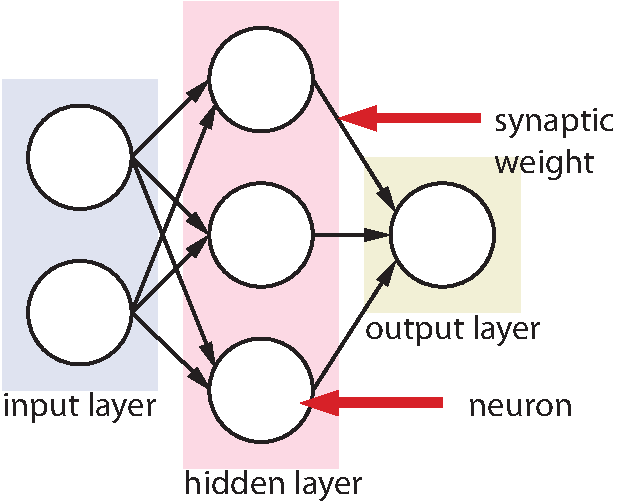
\includegraphics[height=0.30\columnwidth]{figures/ffwdnn.pdf}
		}
		\hspace{2mm} 
		\subfloat[\label{fig:figures_single_neuron} A neuron $j$ with input $x_{k}$ from with synaptic weight $w_{jk}$. The neuron integrates the inputs modulated by their respective weights, and calculates an output with activation function $f$]{	
				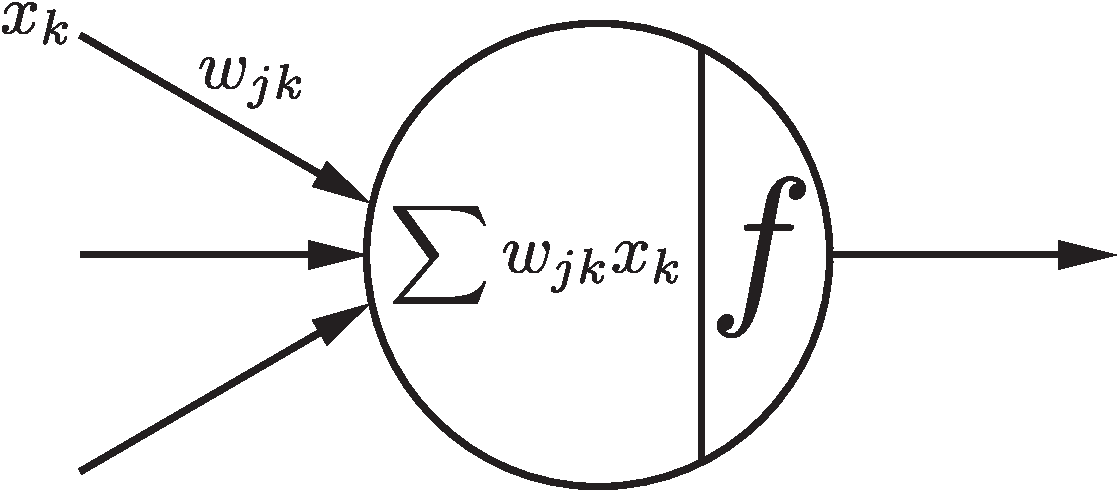
\includegraphics[height=0.20\columnwidth]{figures/single_neuron.pdf}
		}
		\caption{A feedforward neural network and a magnified view of its processing element the neuron}
	\label{fig:figures_ffwdnn_Neuron}	
\end{figure}

\section{Feedforward Neural Networks} % (fold)
\label{sec:feedforward_neural_networks}

In a feedforward neural network only neurons of adjacent layers are interconnected with synaptic weights. Each layer of the neural
network has connections to the next layer and there are no connections oriented backwards. The feedforward neural network begins with an
input layer which may be connected to a hidden layer or directly to an output layer. The first layer is the input layer. It connects
directly to the external environment and captures the input patterns presented to the network. The last layer is the output layer which
produces the output pattern to the external environment. All other layers are considered hidden and may or may not be present.

The processing of a feedforward neural network begins when an external pattern made is copied to the input layer. The neurons of the
input layer communicate the pattern to the following layers through synapses. The pattern is then received by neurons of non-input
layers and modulated by the weight of their connections. We denote weights as $W_{jk}$, where $j$ is the neighbor neuron, and $k$ is the
neuron . Each neuron receives stimulation from other neurons, except the input layer which captures the pattern. Once the inputs are
modulated, they are integrated and an activation value is determined. Often the activation value is just the integration of the
modulated inputs, but may also be a function $F_{i}(a_{i}(t-1), net_{i}(t))$, where $a_{i}(t-1)$ is the activation at the previous time
step and $net_{i}(t)$ is the integration of modulated inputs. (see Algorithm~\ref{alg:feedforward}
)

\begin{algorithm}% [H]
\dontprintsemicolon
\KwIn{Set of inputs from the environment}
\KwOut{Set of output values calculated by the feedforward neural network}
\SetLine
\ForEach{layer from the first non-input layer to the output,}
{
	\ForEach{unit on the current layer,}
	{
		Set the accumulated input value for this unit to zero\;
			\ForEach{ input connection to this unit,} 
			{
				Compute the modulated input across this connection\;
				Add the modulated input to the accumulated input\;
			}
		Convert the accumulated input to its corresponding output\;
		Store the output value for the unit in the layer structure\;
	}
	Return the output values from the top-most layer structure\;
}

\caption{The Feedforward Algorithm (Taken from~\cite{skapura})}
\label{alg:feedforward}
\end{algorithm}

% section feedforward_neural_networks (end)

% section introduction (end)

\section{Data Structure and Algorithms} % (fold)
\label{sec:data_structure_and_algorithms}

To work with the neural network, we represent it using a data structure that is used by the learning algorithms to store the information relevant to neurons and
layers. We examine two different algorithms to train the feedforward neural network. One algorithm is the Back-propagation algorithm and the other is the Root
Mean Square (RMS) Minimization algorithm.

\subsection{Data Structure} % (fold)
\label{sub:data_structure}

We do not have to implement neural networks to study them, it is possible to simulate their execution to solve problems in a computer.
We build data structures in order to represent the neural network. A neural network can be thought of as a directed graph, where the
neurons are nodes, and the synaptic weights are the arcs of the graph. Because we focus on feed-forward networks, our graphs can further
be specified as directed acyclic graphs. These graphs do not require a full matrix to represent all possible connections between the
neurons. Instead we use an array of matrices where each matrix stores the synaptic weights of the departing connections from the current
neuron in the current layer to the neurons of the next layer (see Figures~\ref{fig:figures_ffwdnn2} and
\ref{fig:figures_DataStructure1}).

We may also add an additional free parameter that does not link to other neuron, and has a constant input. We call this parameter the
bias, and it allows the activation functions to translate along the y-axis. We include the bias as one more row of elements for each
matrix that represents connections between neurons (see Figure~\ref{fig:figures_ffwdnn3} and \ref{fig:figures_DataStructure2}).

\begin{figure}[]
	\centering
		\subfloat[\label{fig:figures_ffwdnn2}]{	
				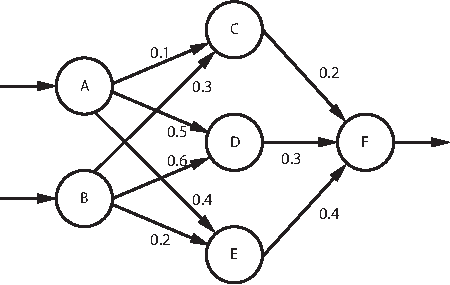
\includegraphics[width=0.45\columnwidth]{figures/ffwdnn2.pdf}
		}
		\hspace{2mm}
		\subfloat[\label{fig:figures_ffwdnn3}]{	
				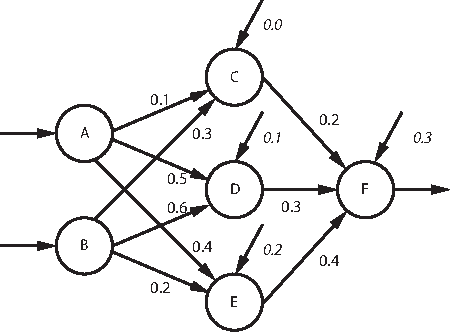
\includegraphics[width=0.45\columnwidth]{figures/ffwdnn3.pdf}
		}

		\subfloat[\label{fig:figures_DataStructure1}]{	
				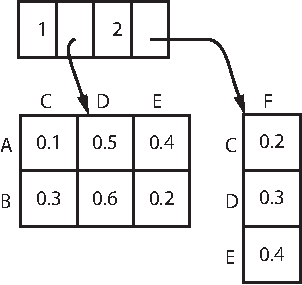
\includegraphics[width=0.35\columnwidth]{figures/DataStructure1.pdf}
		}
		\hspace{8mm} 
		\subfloat[\label{fig:figures_DataStructure2}]{	
				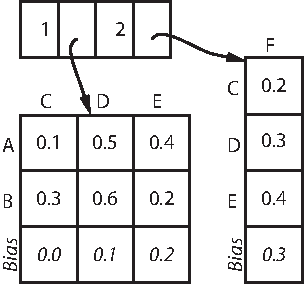
\includegraphics[width=0.35\columnwidth]{figures/DataStructure2.pdf}
		}
		\caption{Feedforward neural networks (a and b) with their corresponding computer representation (c and d). Figures~\ref{fig:figures_ffwdnn2} and \ref{fig:figures_DataStructure1} represent a neural network without bias parameters. Figures~\ref{fig:figures_ffwdnn3} and \ref{fig:figures_DataStructure2} represent a neural network with bias parameters}
	\label{fig:figures_ffwdnn_DS}	
\end{figure}

% subsection data_structure (end)

\subsection{Backpropagation training algorithm} % (fold)
\label{sub:backpropagation_training_algorithm}

Back-propagation is a method of supervised learning. It is used to train our feedforward neural network. To use the back-propagation
algorithm we provide it with both example inputs and target outputs. The outputs generated by the neural network are then compared
against the target outputs of the given example. Using the target outputs, the back-propagation training algorithm then calculates
errors and adjusts the weights of the various layers backwards from the output layer to the input layer.

Back-propagation is often used to train feedforward neural networks but it can also be used to train other types of networks, and
likewise feedforward networks may be trained with other methods. In this report, we only examine back-propagation when it is used to
train a feedforward neural network. Algorithm~\ref{alg:backpropagation} illustrates in further detail Back-propagation.

\begin{algorithm}% [H]
\dontprintsemicolon
\KwIn{Set of examples $E$}
\tcc{$e$ is a single example} 
\tcc{$I(e)$ set of inputs in a single example}
\tcc{$T(e)$ set of target outputs for a given example}
\tcc{$O(e)$ are the target outputs of the example}
\tcc{Each iteration of this loop we an epoch}

% \KwOut{Set of output values calculated by the feedforward neural network}
\SetLine
\ForEach{ example $e$ in a set of examples $E$}
{
	Calculate $O(e)$ for $I(e)$ with feedforward (refer to Algorithm~\ref{alg:feedforward})\;
	Call function \textbf{CalculateOutputDeltas}($O(e)$, $T(e)$)\;
	Call function \textbf{CalculateInternalDeltas}\;
	Call function \textbf{UpdateWeights}\;
}

\textbf{CalculateOutputDeltas($O(e)$, $T(e)$):}

Get output values $O(e)$ from the output layer neurons\;
\ForEach{ individual output value $O(e)_i$ }
{
	Calculate error $\epsilon$ as $O(e)_i$ - $T(e)_i$\;
	Calculate \textbf{$\delta_{O(e)_{i}} = \partial{f(O(e)_{i})}  \times \epsilon $}\;
	Add $\delta_{O(e)_{i}}$ to set of deltas $\Lambda$
}  

\textbf{CalculateInternalDeltas:}

Let $\Lambda_{i+1}$ be the next layer's set of deltas\;
\ForEach{ non-output layer $i$ from the penultimate to the first}
{
	\ForEach{ neuron $j$ in this layer } 
	{
	Initialize error $\epsilon$ as $0.0$\;
		\ForEach{ neuron $k$ of the next layer} 
		{
			Calculate $\epsilon$ as $\epsilon + \Lambda_{i+1,k} W_{ijk}$\;
		}
		$\Lambda_{i,j} = \partial{f( \epsilon \times \mbox{neuron } j\mbox{'s output} )}$\;
	}
} 

\textbf{UpdateWeights:}

\tcc{$\eta$ is the learning rate}
\ForEach{ layer $i$ }
{
	\ForEach{ neuron $j$ in this layer } 
	{
		\ForEach{ neuron $k$ of the next layer} 
		{
			Calculate $\Delta W_{ijk}$ as $\Lambda_{i,j} \times \mbox{neuron } j\mbox{'s output}$\;
			$W_{ijk} \leftarrow \eta \times \Delta{W_{ijk}}   $\;
		}
	}
} 

\caption{The Back-propagation Algorithm }
\label{alg:backpropagation}
\end{algorithm}

\begin{figure}[]
	\centering
		\subfloat[\label{fig:figures_backpgtn1}]{	
				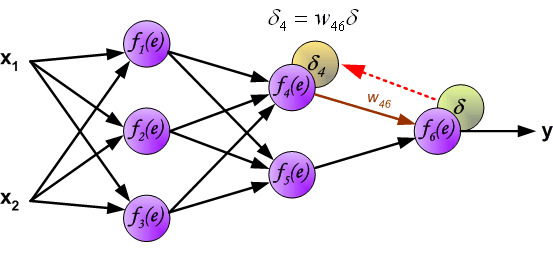
\includegraphics[width=0.49\columnwidth]{figures/backpgtn1.png}
		}
		\subfloat[\label{fig:figures_backpgtn2}]{	
				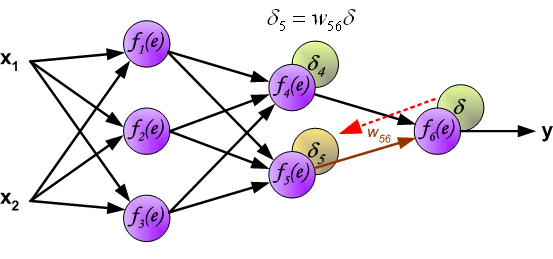
\includegraphics[width=0.49\columnwidth]{figures/backpgtn2.png}
		}
		
		\subfloat[\label{fig:figures_backpgtn3}]{	
				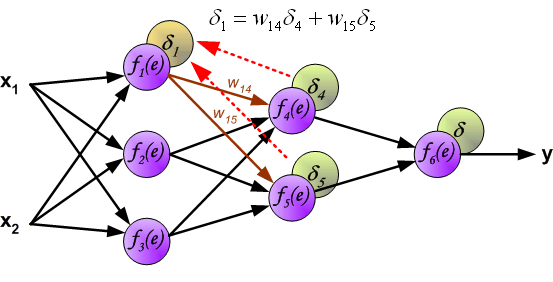
\includegraphics[width=0.49\columnwidth]{figures/backpgtn3.png}
		}
		\subfloat[\label{fig:figures_backpgtn4}]{	
				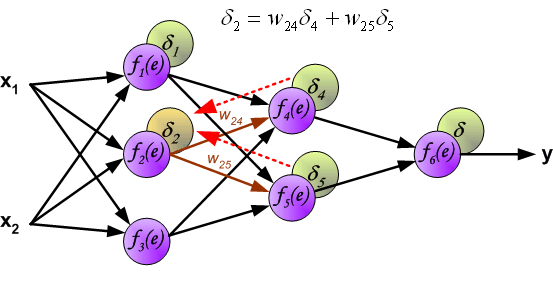
\includegraphics[width=0.49\columnwidth]{figures/backpgtn4.png}
		}
		
		\subfloat[\label{fig:figures_backpgtn5}]{	
				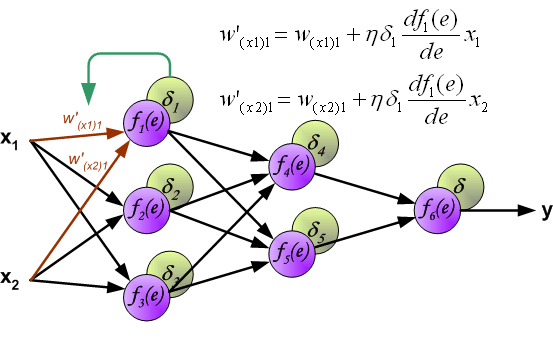
\includegraphics[width=0.49\columnwidth]{figures/backpgtn5.png}
		}
		\subfloat[\label{fig:figures_backpgtn6}]{	
				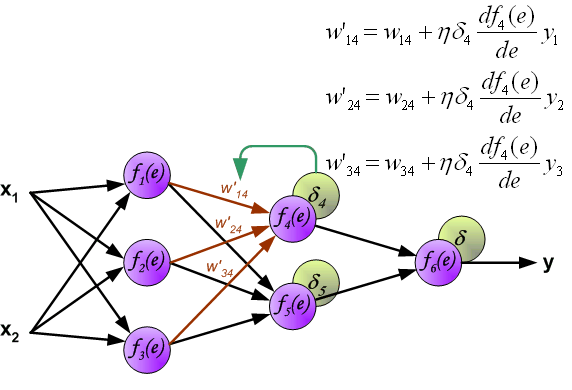
\includegraphics[width=0.49\columnwidth]{figures/backpgtn6.png}
		}
		
		\caption{An illustration of the Back-propagation algorithm. (Taken from \cite{vlsibackp_t})}
	\label{fig:figures_backpgtn}	
\end{figure}

% subsection backpropagation_training_algorithm (end)

\subsection{RMS Minimization Algorithm} % (fold)
\label{sub:rms_minimization_algorithm}

Another algorithm we use to train the feedforward neural network is the Root Mean Square (RMS) Minimization algorithm (see
Algorithm~\ref{alg:RMSminimization} ). For this algorithm we also provide example inputs and target outputs. We run the feedforward
algorithm with each example generating the corresponding outputs of the neural network. After generating the outputs we calculate the
root mean square between outputs given by the neural network and target output provided by the example. We keep this calculation as
$\mbox{RMS}_\mbox{old}$. Next, a small change is made to one of the weights of the neural network, and the feedforward algorithm is
called again to calculate new outputs for the neural network. We again, take the root mean square between outputs and targets which we
call $\mbox{RMS}_\mbox{new}$. We then calculate a slope by taking the difference between $\mbox{RMS}_\mbox{old}$ and
$\mbox{RMS}_\mbox{new}$, and divide by the change we made to the weight.

We use this slope to determine what change needs to be made to improve the RMS between the output of our network and the target from the
example. Unlike the back-propagation method, this method performs a $num(E)$ feedforward passes, where $num(E)$ is the number of
examples used to train the network.

\begin{algorithm}% [H]
\dontprintsemicolon
\KwIn{Set of examples $E$, constants $\alpha$ and $\epsilon$}
\tcc{Each iteration of this loop we will call an epoch}
Set $\Delta W$ to $0.01$\;
\SetLine
\ForEach{layer $i$ from the first non-input layer to the output,}
{
	\ForEach{layer $i$ from the first non-input layer to the output,}
	{
		\ForEach{neuron $j$ on the current layer,}
		{
				\ForEach{ connection $k$ to a neuron of the next layer,} 
				{
					Calculate $\mbox{RMS}_{\mbox{o}}$ as \textbf{CalculateRMS}($E$)\;
					Set $W_{ijk}$ to $W_{ijk}$ + $\Delta W$\;
					Calculate $\mbox{RMS}_{\mbox{n}}$ as \textbf{CalculateRMS}($E$)\;
				
					Calculate $\Delta RMS$ as $ \frac{\mbox{RMS}_{\mbox{n}}-\mbox{RMS}_{\mbox{o}}}{\Delta W} $\;
				
					\If{ $\Delta RMS \neq 0.0 $}{
					  Calculate $\Delta W_{ijk}$ as $\alpha \times \Delta W_{ijk} - \epsilon \times \Delta RMS$\;
					  Calculate $W_{ijk}$ as $W_{ijk} + \Delta W_{ijk}$\;
					}
				}
		}
	}
}

\textbf{CalculateRMS($E$)}:
\dontprintsemicolon
\tcc{$e$ is a single example} 
\tcc{$I(e)$ set of inputs in a single example}
\tcc{$T(e)$ set of target outputs for a given example}
\tcc{$O(e)$ are the target outputs of the example}
Set $\epsilon$ to $0.0$\;
\ForEach{example $e$ in the set of examples $E$} 
{
	$O(e)$ $\leftarrow$  Call feedforward algorithm with $I(e)$ (see Algorithm~\ref{alg:feedforward})\;
	\ForEach{ output $O(e)_i$ obtained from the neural network }
	{
		Calculate $\epsilon$ as $\epsilon + (O(e)_{i} - T(e)_{i})^{2}$\;
	} 
	
}
\Return $\frac{\epsilon}{\mbox{num}(E) - 1}$\; \tcc*{ $\mbox{num}(E)$ is the total number of examples in $E$}
\vspace{5mm} 
\caption{The RMS Minimization Algorithm}
\label{alg:RMSminimization}
\end{algorithm}


% subsection rms_minimization_algorithm (end)

% section data_structures_and_algorithms (end)

\section{Experiments and Results} % (fold)
\label{sec:results}

A set of system experiments are performed where we test the RMS and back-propagation training methods. We compare the time complexity
between both training methods as well as their accuracy after training is completed. The set of examples to train the network are
generated by taking two numerical inputs and adding them to generate the expected output. This data is normalized so that its range is
between -1 and 1. The feedforward neural network is configured with $2$ neurons in the input layer, $3$ in the middle layer and $1$ in
the output layer. The neurons in the middle layer use a hyperbolic tangent activation function, and the neurons in the output layer use
a linear function. In our procedures we change different parameters of the neural network, and observe the behavior in time complexity
and accuracy.

\subsection{Time Complexity} % (fold)
\label{sub:time_complexity}

We tested the time complexity of both algorithms in different aspects. We look at how time changed when we varied the number of neurons
in the middle layer. Time grew linearly for the back-propagation algorithm when the number of neurons is varied whereas in the RMS
Minimization algorithm it grows quadratically.

Looking at the time complexity analytically we count the number of operations made by both algorithms. To determine the number of
operations performed at each epoch of the learning algorithm we count the weights between the layers of the neural network. To do this
we consider that the number of weights between two layers of neurons is the product between the total neurons in two adjacent layers.
Therefore the total number of weights for the entire network is $\sum_{i=0}^{n-1}N_{i}N_{i+1}$ where $N_{i}$ is the number of neurons in
each layer, and $n$ is the total number of layers. For the back-propagation algorithm, the number of operations in a single epoch
depends on the number of weights and biases. For the biases we count one bias for each neuron that is not in the input layer.

For the back-propagation algorithm we run the feedforward algorithm once, and then calculate an error for the first output layer. The
error is then propagated backwards to each layer where each needed change to the weights is calculated. After this propagation the
weights are added modified. All this steps require the same set of $n$ operations for each weight as it propagates backwards, and $n$
operations as it makes the changes to the weights. Therefore this algorithm has a linear complexity $O(n)$ with respect to the number of
neurons in the middle layer.

For the RMS algorithm the number of operations in a single epoch depends on both the number of weights and the number of is squared
because we run the feedforward algorithm for each change we do on a single weight.


\begin{figure}[]
	\centering
		\subfloat[\label{fig:docs_graphs_TimeNrns}]{	
				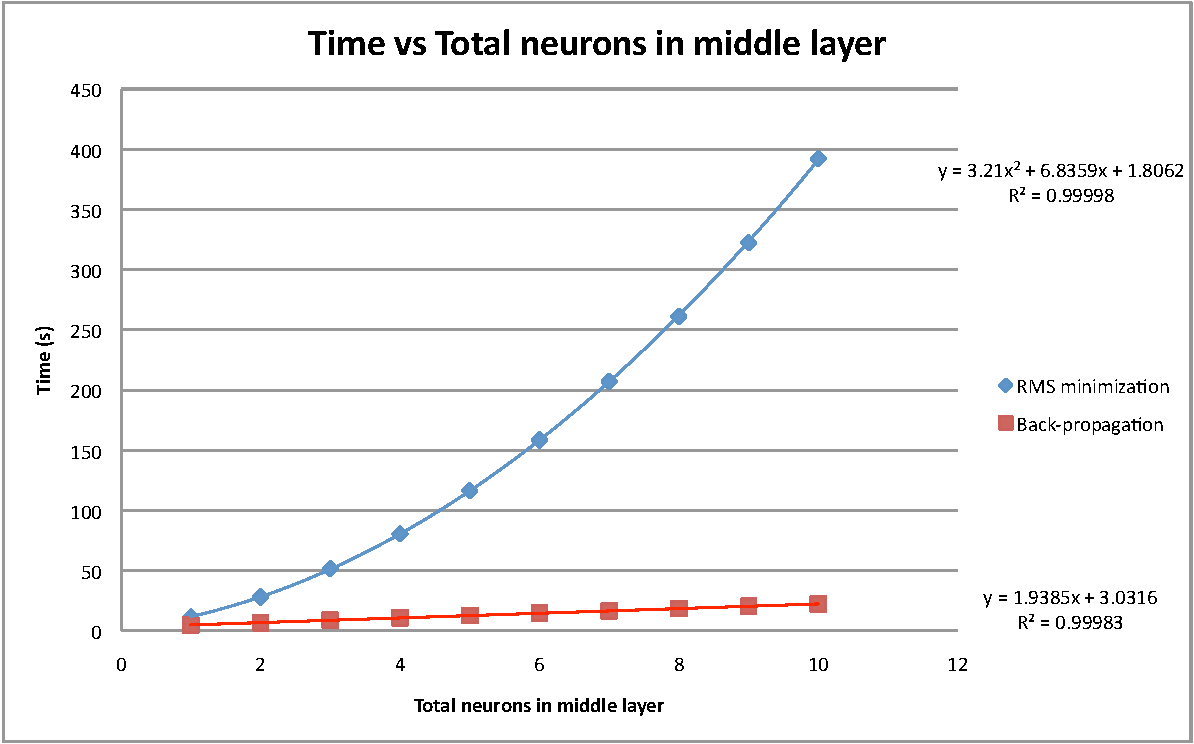
\includegraphics[width=0.60\columnwidth]{../docs/graphs/TimeNrns.pdf}
		}                                           
		   
		\subfloat[\label{fig:docs_graphs_TimeItrns}]{  
				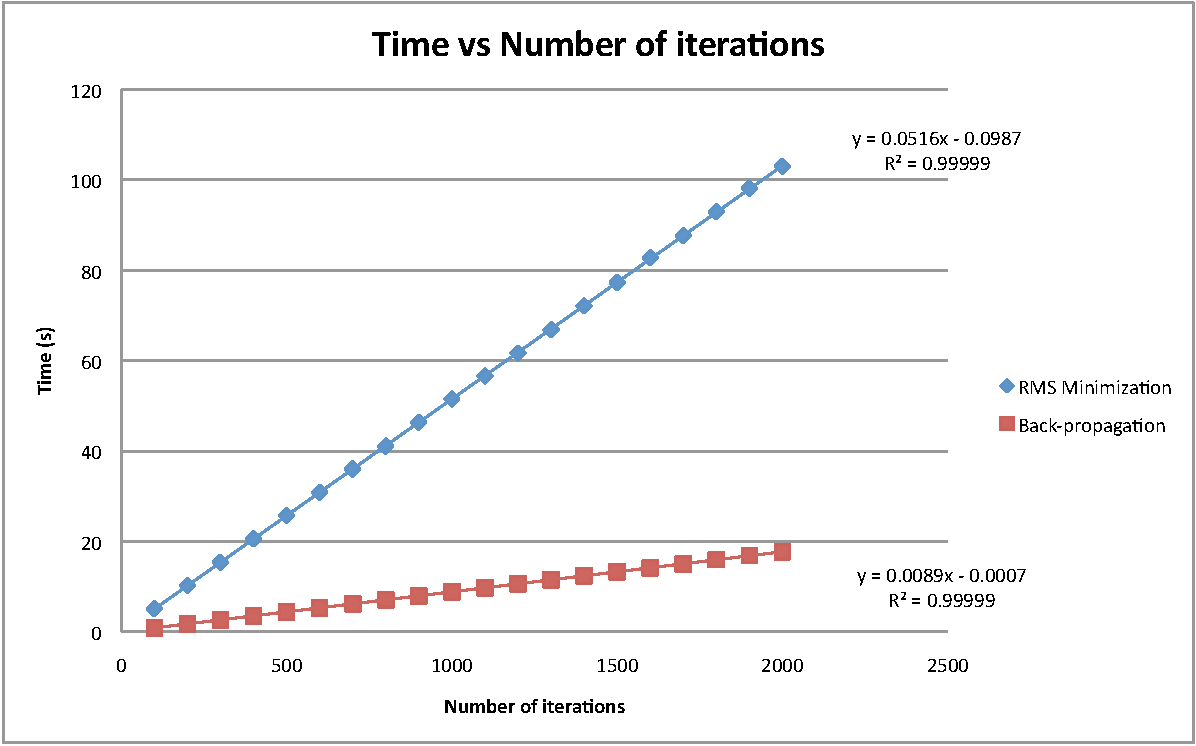
\includegraphics[width=0.60\columnwidth]{../docs/graphs/TimeItrns.pdf}
		}
		
		\subfloat[\label{fig:docs_graphs_TimeSmpls}]{  
				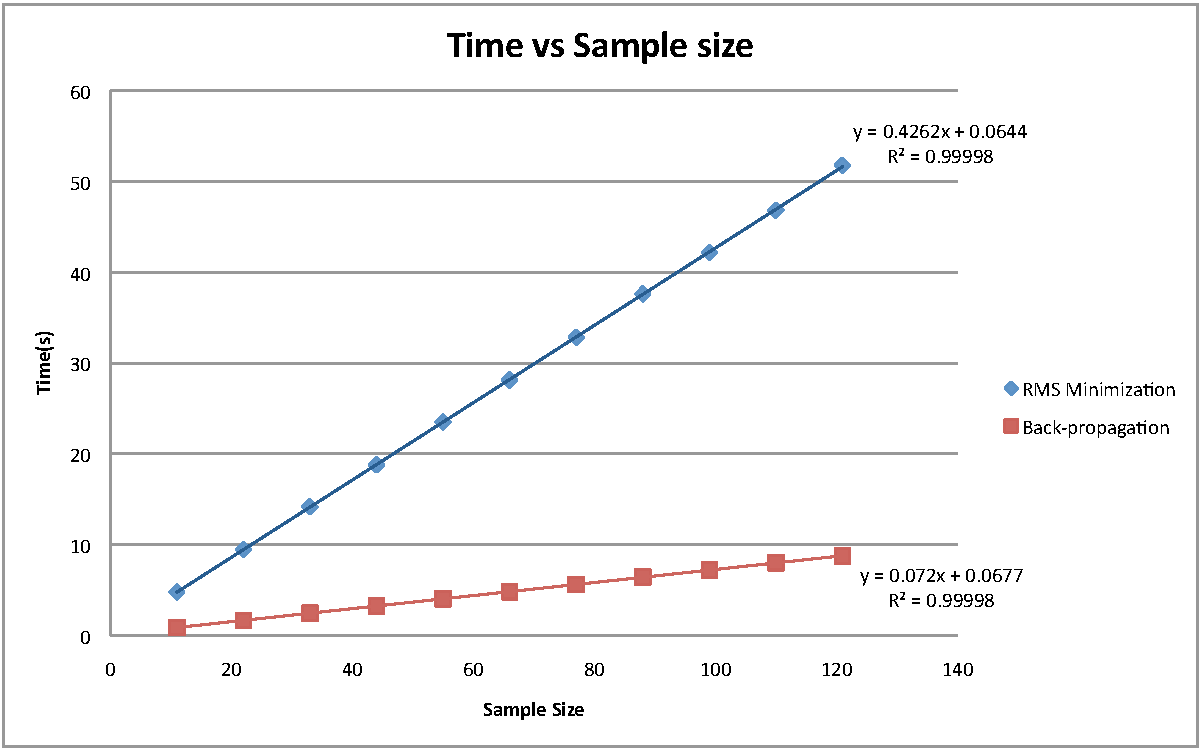
\includegraphics[width=0.60\columnwidth]{../docs/graphs/TimeSmpls.pdf}
		}
		\caption{Comparison in times between back-propagation and RMS minimization training algorithms. In Figure~\ref{fig:docs_graphs_TimeNrns} the the number of neurons in the middle layer is varied and time is measured. In Figure~\ref{fig:docs_graphs_TimeItrns} the number of iterations is varied. In Figure~\ref{fig:docs_graphs_TimeSmpls} the size of the sample is varied }
	\label{fig:docs_graphs_Time}	
\end{figure}



% subsection time_complexity (end)

% section results (end)

\section{Conclusion} % (fold)
\label{sec:conclusion}

The Backpropagation algorithm has time complexity within $O(n)$, which is faster than the RMS Minimization algorithm with a time
complexity of $O(n^{2})$ when varying the number of neurons in the middle layer. 

The Backpropagation algorithm reached a smaller error for the simple examples that the RMS Minimization algorithm.

As observed in some results, the neural network may get stuck in local minima unable to arrive to better solutions. We noticed this in
both the Backpropagation and RMS Minimization algorithms.

% section conclusion (end)	
    
\bibliographystyle{plain}
\bibliography{bib/eds}
\end{document} 